\documentclass[a4paper,10pt,fleqn]{article}

\usepackage{a4wide,amsmath,amsthm,amssymb,bbm,fancyhdr}
\usepackage{ifthen,color,enumerate,comment,dsfont,pdfsync,framed,todonotes,enumitem}

\newcommand{\titre}[1]{\textbf{\textsc{#1}}}

\RequirePackage[T1]{fontenc}

\usepackage[latin1]{inputenc}
\usepackage{graphicx}
\usepackage{dsfont}
\usepackage{enumitem}
\newcommand{\eqsp}{\,}
\newcommand{\R}{\ensuremath{\mathbb{R}}}
\newcommand{\calF}{\mathcal{F}}
\newcommand{\rmd}{\mathrm{d}}
\newcommand{\N}{\mathbb{N}}
\newcommand{\rset}{\ensuremath{\mathbb{R}}}
\renewcommand{\P}{\ensuremath{\operatorname{P}}}
\newcommand{\bP}{\mathbb{P}}
\newcommand{\E}{\ensuremath{\mathbb{E}}}
\newcommand{\rme}{\ensuremath{\mathrm{e}}}
\newcommand{\calH}{\ensuremath{\mathcal{H}}}
\newcommand{\xset}{\ensuremath{\mathsf{X}}}
\newcommand{\V}{\ensuremath{\mathbb{V}}}
\newcommand{\Sb}{\ensuremath{\mathbb{S}}}
\newcommand{\gaus}{\ensuremath{\mathcal{N}}}
\newcommand{\HH}{\ensuremath{\mathcal{H}}}
\newcommand{\F}{\ensuremath{\mathcal{F}}}
\newcommand{\W}{\ensuremath{\mathcal{W}}}
\newcommand{\X}{\ensuremath{\mathcal{X}}}
\newcommand{\1}{\ensuremath{\mathbbm{1}}}
\newcommand{\dlim}{\ensuremath{\stackrel{\mathcal{L}}{\longrightarrow}}}
\newcommand{\plim}{\ensuremath{\stackrel{\mathrm{P}}{\longrightarrow}}}
\newcommand{\PP}{\ensuremath{\mathbb{P}}}
\newcommand{\p}{\ensuremath{\mathbb{P}}}
\newcommand{\eps}{\varepsilon}
\newcommand{\bE}{\mathbb{E}}
\newcommand{\pa}[1]{\left(#1\right)}
\newcommand{\hatk}{\widehat K}
\newcommand{\f}{\varphi}
\newcommand{\Id}{\textsf{Id}}
\newcommand{\bfU}{\mathbf{U}}
\newcommand{\bfX}{\mathbf{X}}
\newcommand{\bfs}{\mathbf{\Sigma}}
\newcommand{\bfA}{\mathbf{A}}
\newcommand{\bfV}{\mathbf{V}}
\newcommand{\bfB}{\mathbf{B}}
\newcommand{\bfI}{\mathbf{I}}
\newcommand{\bfD}{\mathbf{D}}
\newcommand{\bfK}{\mathbf{K}}
\newcommand{\argmin}{\mathop{\textrm{argmin}}}
\newcommand{\argmax}{\mathop{\textrm{argmax}}}
\newcommand{\crit}{\mathop{\textrm{crit}}}
\newcommand{\C}{\mathcal{C}}
\newcommand{\pc}{\pi_{\mathcal{C}}}


% Style


\newtheorem{theorem}{Theorem}


\begin{document}

%\noindent Machine learning \hfill ISUP - Sorbonne Universit\'e \\
% 2022-2023

\noindent\hrulefill

\begin{center}
\textsc{Introduction to Bayes classification}
\end{center}
\hrulefill

\medskip


\section{Warm-up: Bayes classifier for scalar Gaussian mixtures}
Let $(X_i,Y_i)_{1\leqslant i\leqslant n}$ be independent variables in $\mathbb{R}\times \{0,1\}$. Assume that  $\mathbb{P}(Y_1 = 0) = 1/2$. Assume also that the distribution of $X_1$ given $\{Y_1= 0\}$ (resp. $\{Y_1= 1\}$) is Gaussian with mean $\mu_0$ (resp. $\mu_1$) and variance $1$. The probability density function of $X_1$ is written $g$. Write
$$
g_0: x \mapsto (2\pi)^{-1/2}\exp(-(x-\mu_0)^2/2)\quad\mathrm{and} \quad g_1: x \mapsto (2\pi)^{-1/2}\exp(-(x-\mu_1)^2/2)\eqsp.
$$
\begin{figure}[h!]
\begin{center}
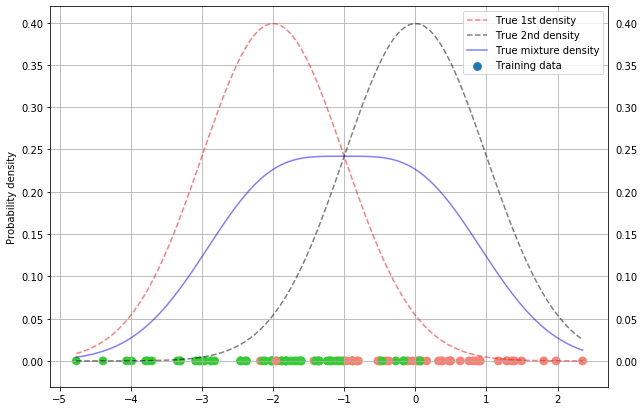
\includegraphics[scale=0.3]{mu0_mum2.png}
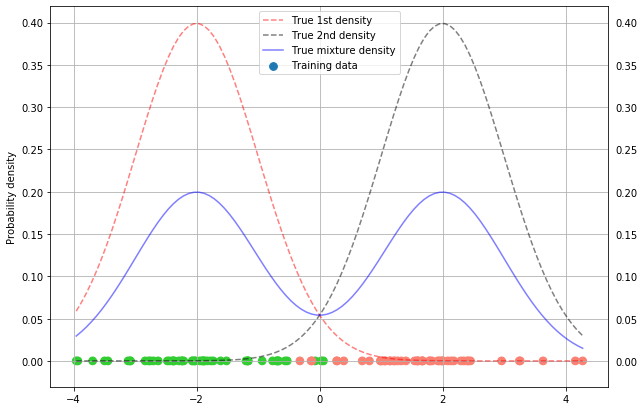
\includegraphics[scale=0.3]{mu2_mum2.png}
\caption{Samples and density when   $\mu_0 = -2$ et $\mu_1 = 0$ (left) and $\mu_0 = -2$ and $\mu_1 = 2$ (right).}
\end{center}
\end{figure}

\begin{enumerate}
\item Provide an expression of a classifier $h_*$ minimizing $h \mapsto \bP(h(X)\neq Y)$.

\item Using Bayes rule, show that  $h_*$ depends only on $g_1/g_0$.

\item Show that the Bayes classifier uses the mean between  $\mu_0$ and  $\mu_1$ to classify samples.

\end{enumerate}



\section{Bayes classifier}
\subsection{Uniform distributions}
Assume that $(X,Y)\in\mathbb{R}\times\{0,1\}$ is defined on $(\Omega,\mathcal{F},\mathbb{P})$ with $\mathbb{P}(Y=1) = \pi \in(0,1)$.  Assume that conditionally on $\{Y=0\}$ (resp. $\{Y=1\}$) $X$ has a uniform distribution on $[0,\theta]$ with $\theta\in(0,1)$ (resp. on $[0,1]$). Compute $\eta(X) = \mathbb{P}(Y=1 |X)$.

\subsection{Weighted risk}
Assume that $(X,Y)\in\mathbb{R}\times\{0,1\}$ is defined on $(\Omega,\mathcal{F},\mathbb{P})$. Using $\omega_0, \omega_1 >0$, with $\omega_0+\omega_1 = 1$, we  consider the weighted risk:
$$
\mathsf{R}(h) = \bE[2\omega_Y \mathds{1}_{Y\neq h(X)}]\,.
$$
Compute a classifier $h_*$ minimizing $h\mapsto \mathsf{R}(h)$ and $\mathsf{R}(h_*)$.


\section{Additional exercises}

\subsection{Bayes classifier: excess risk}
Let $(X,Y)\in\rset^d\times\{0,1\}$ be random variables defined on the same probability space $(\Omega,\calF,\bP)$.
For any classifier $h:\mathcal{X}\to \{0,1\}$, define its classification error by
$$
\mathsf{R}(h)=\bP(Y\neq h(X))\eqsp.
$$
The classifier $h_*$ defined by:
$$
h_{*}(x)={\rm sign}(\eta(x)-1/2)\eqsp,
$$
where
$$
\eta(X) = \bP(Y=1|X)\eqsp,
$$
minimizes $h\mapsto \mathsf{R}(h)$.
\begin{enumerate}
\item Prove that 
$$
\mathsf{R}(h_*) = \mathbb{E}\left[\eta(X) \wedge (1-\eta(X))\right]\leqslant \frac{1}{2}\eqsp.
$$
\item Prove that for all classifiers $h$, the excess risk is given by
$$
\mathsf{R}(h)  - \mathsf{R}(h_*) = \mathbb{E}\left[\left|1-2\eta(X)\right|\left|h(X) - h_*(X)\right|\right]\eqsp.
$$
\end{enumerate}



\subsection{Plug-in classifier}
Let $(X,Y)\in\rset^d\times\{-1,1\}$ be random variables defined on the same probability space $(\Omega,\calF,\bP)$.
For any classifier $h:\mathcal{X}\to \{-1,1\}$, define its classification error by
$$
\mathsf{R}(h)=\bP(Y\neq h(X))\eqsp.
$$
The classifier $h_*$ defined by:
$$
h_{*}(x)={\rm sign}(\eta(x)-1/2)\eqsp,
$$
where
$$
\eta(X) = \bP(Y=1|X)\eqsp,
$$
minimizes $h\mapsto \mathsf{R}(h)$. Given $n$ independent couples $\{(X_i,Y_i)\}_{1\leqslant i \leqslant n}$ with the same distribution as $(X,Y)$, an empirical surrogate for $h_{*}$ is obtained from a possibly nonparametric estimator $\widehat \eta_n$ of $\eta$:
$$
\widehat h_n: x\mapsto {\rm sign}(\widehat \eta_n(x)-1/2)\eqsp.
$$
\begin{enumerate}
\item Prove that for any classifier $h:\mathcal{X}\to \{-1,1\}$,
$$
\bP(Y\neq h(X)|X) = (2\eta(X)-1)\1_{h(X)=-1}+1-\eta(X)
$$
and
$$
\mathsf{R}(h)-\mathsf{R}(h_{*})=2\bE \left[\left|\eta(X)-\frac{1}{2}\right|\eqsp\1_{h(X)\neq h_*(X)}\right]\eqsp.
$$
\item Prove that 
$$
|\eta(x)-1/2|\1_{\widehat h_n(x)\neq h_{*}(x)}\leqslant |\eta(x)-\widehat \eta_n(x)|\1_{\widehat h_n(x)\neq h_{*}(x)}\eqsp,
$$
where
$$
\widehat h_n:x \mapsto{\rm sign}(\widehat \eta_n(x)-1/2)\eqsp.
$$
Deduce that 
$$
\mathsf{R}(\widehat h_n)-\mathsf{R}(h_*)\leqslant  2 \bE[|\eta(X) - \widehat \eta_n(X)|^2]^{1/2}\eqsp.
$$
\end{enumerate}



\end{document}